This section will explain the functions to read the sensors data from a AM2302. Due to the specific GPIO function in Azure Sphere, it may not able to read the one-wire sensor, such as the AM2302. To have a work around, the sensor connects to an Arduino device, and send the sensor data through UART to Azure Sphere. 

This section assume you already have:
\begin{itemize}
    \item Your Azure Sphere device is connected to your PC
    \item You have completed all the steps to \autoref{sec:sim_app}
    \item You have git command installed in a PC.
    \item You have Visual Studio 2017
    \item You have Arduino IDE
\end{itemize}

\subsection{Connect Azure Sphere to Arduino and AM2302}
The Azure Sphere communicates with Arduino through UART. The UART pins on Azure Sphere are PIN1(RXD0) and PIN3(TXD0) in Header 2. The wirings are:  
\begin{itemize}
    \item Arduino TX(PIN1)->AzureSphere RXD0(Header2, PIN1)
    \item Arduino RX(PIN0)->AzureSphere TXD0(Header2, PIN3)
\end{itemize}

The diagram shows how to connect them. 
\begin{figure}[h]
    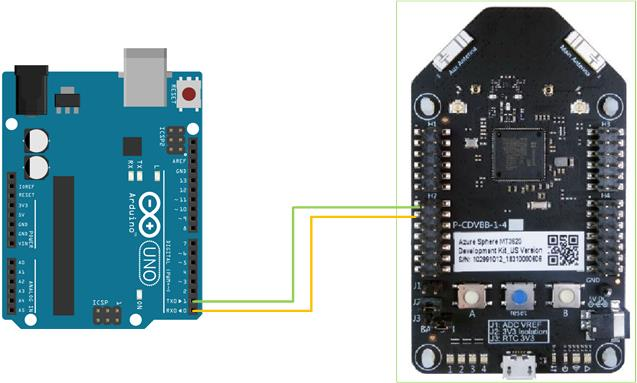
\includegraphics[scale=0.7]{AStoAD.jpg}
\end{figure}

Connecting Arduino to the AM2302 is fairly straight forward, there are three cables to AM2303, red cable to VCC(3.3v/5v), black cable to GND and yellow cable is the signal out, in this project it connects to PIN2.
The diagram shows how to connect the Arduino with AM2302:
\begin{figure}[h]
    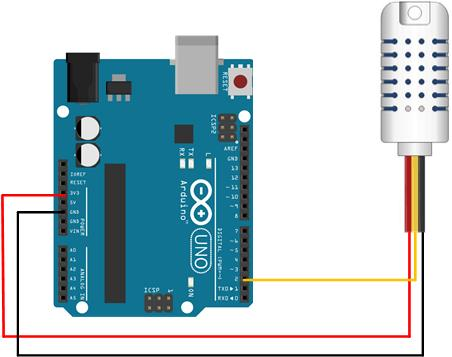
\includegraphics[scale=0.6]{ADtoAM2302.jpg}
\end{figure}

\subsection{Clone the code from Github}
The code can be download from Github using following command:
\begin{lstlisting}[language=bash]
git clone https://github.com/jianyuanMa/AzureSphereDHT22.git
\end{lstlisting}

\subsection{Some Explanations about the project}
The project has two parts. First part is the Arduino read the sensor data periodically and send it to the UART while the Azure Sphere receives the data as the second part.

\subsubsection{Read Sensor Data in Arduino}
Open Arduino IDE in the Start menu and open the file UartAM2302.ino in the folder ArduinoCode. The sensor reading uses the library from Adafuit. To install the library, select \textbf{Sketch>Include Library>Manage Libraries} in the dropdown menu. 

Enter "DHT" in the search field and look through the list for “DHT sensor library by Adafruit.” Click the “Install” button, or “Update” from an earlier version.
\begin{figure}[h]
    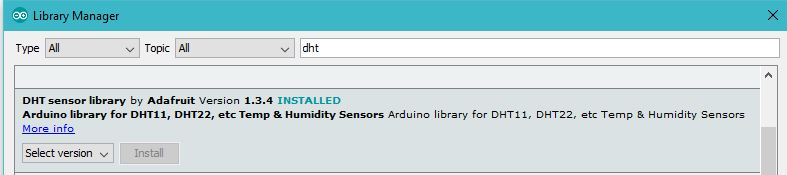
\includegraphics[scale=0.6]{DHTLibary.JPG}
\end{figure}

You also need to install the Adafruit\_Sensor library, which is also available in the Arduino Library Manager.
\begin{figure}[h]
    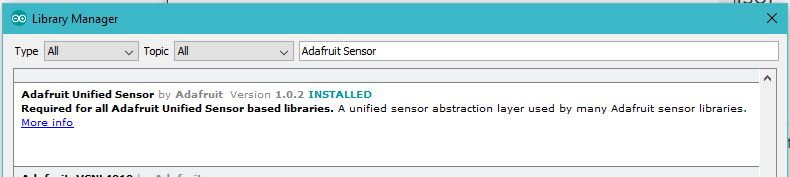
\includegraphics[scale=0.6]{AdafruitUnifiedSensor.JPG}
\end{figure}

\subsubsection{Communicate through UART}
The second part is communication between the Arduino and Azure Sphere through UART. Open Visual Studio 2017 and select \textbf{File->Open->Project/Solution}. In the open dialogue, navigate to the Git repository we just downloaded and select the file "AzureArdruino.sln" to open the Visual Studio Project.

This project is referenced to the \textbf{UART Sample for MT3620 RDB(Azure Sphere)}, you find it by select \textbf{Fild>New Poject>Visual C++>Cross Platform>Azure Sphere}.

To use the UART read function, it needs to include the "applibs/uarts.h" library. The funtion "UartEventHandler" reads the messages whenever they have been sent from the Arduino. Since we know the messages are the sensor data from AM2302 in an array format {humidity,temperature}. We can easily convert each message into the actual numbers and ready for uploading to the cloud. The function "charArrayToNumbers" helps to achieve that.

\subsection{Test the Output}
\begin{enumerate}
    \item Connect Arduino to a PC and start the Arduino IDE. Then open the UartAM2302.ino.
    
    \item Select \textbf{Tools>Port} then looking for the port with the description \textbf{Arduino/Genuino Due}.
    
    \item Click Upload \inlinegraphics{UploadBTArduino.JPG} in the tool bar. If you see the output similar to the following, it means the program has been successfully uploaded to the Arduino.
    \begin{lstlisting}[language=bash]
Sketch uses 5682 bytes (17%) of program storage space. Maximum is 32256 bytes.
Global variables use 191 bytes (9%) of dynamic memory, leaving 1857 bytes for local variables. Maximum is 2048 bytes.
    \end{lstlisting}
    
    \item Connect the Azure Sphere to a PC. Prepare the board to enable the debug from a PC.
    \begin{lstlisting}[language=bash]
    azsphere device prep-debug
    \end{lstlisting}
    
    \item Open the \textbf{AzureArduino.sln} in Visual Studio 2017. Then select the \textbf{Remote GDB Debugger} in the tools bar to start the debug process.
    
    \item You should be to see the output in the Output window like:
    \begin{lstlisting}[language=bash]
Remote debugging from host 192.168.35.1
UART application starting.
Opening MT3620_RDB_LED2_RED.
Humidiy 18.70, Temperature 22.10
Humidiy 18.70, Temperature 22.10
......
    \end{lstlisting}
    
\end{enumerate}